\section{Analyses \& Findings}

Given a set of papers' citations (total number $N$), we count the number ($n_\text{HCI}$) of citations that came from the core HCI venues.
Then, \xin is simply $1-n_\text{HCI}/N$.
Specifically, for a paper that cites an HCI paper, we use simple keyword matching to determine whether that paper was published in one of the core HCI venues.

\fg{fig1}{fig1}{1.0}{\xin of more recently published HCI papers (CHI, UIST, and CSCW) have a lower \xin than earlier papers'.}

\fg{fig2}{fig2}{1.0}{If only considering HCI papers that have existed for at least five years, the more recently-published papers' \xin is still lower.}

\subsection{\xin~ of HCI Papers Published Over the Years}
We calculate the \xin of each year's HCI papers (\eg 11 years of UIST papers between 2010 and 2020), as shown in \fgref{fig1}.
Each point in \fgref{fig1} is the \xin value based on citations of that year's published HCI papers up to when the data was collected (January 2023).
We can see that all three HCI venues' papers have an decreasing \xin over the years.
In other words, HCI papers published later tend to be cited less often by papers outside of the core HCI venues.

One might question that, since citation count is also a function of time, the more recent HCI papers might be disadvantaged simply because they have not existed long enough to attract citations.
To resolve this doubt, we perform the next analysis.

\begin{figure}[t]
    \centering
    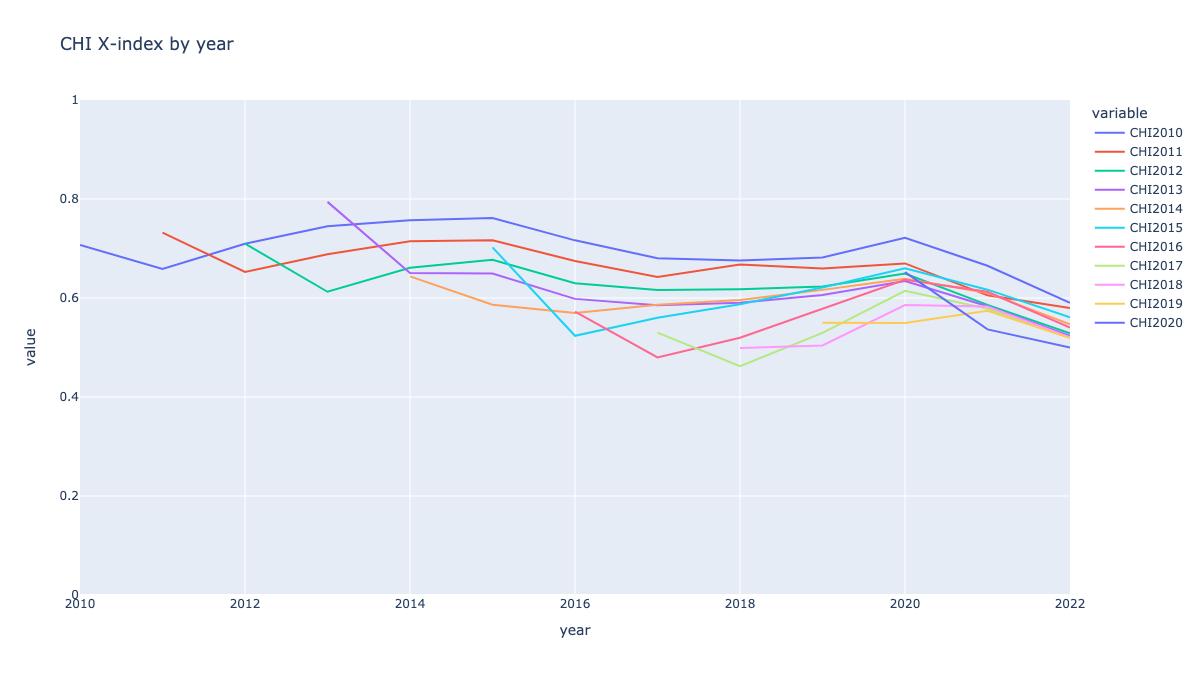
\includegraphics[width=\columnwidth]{figures/fig3_CHI.png}
    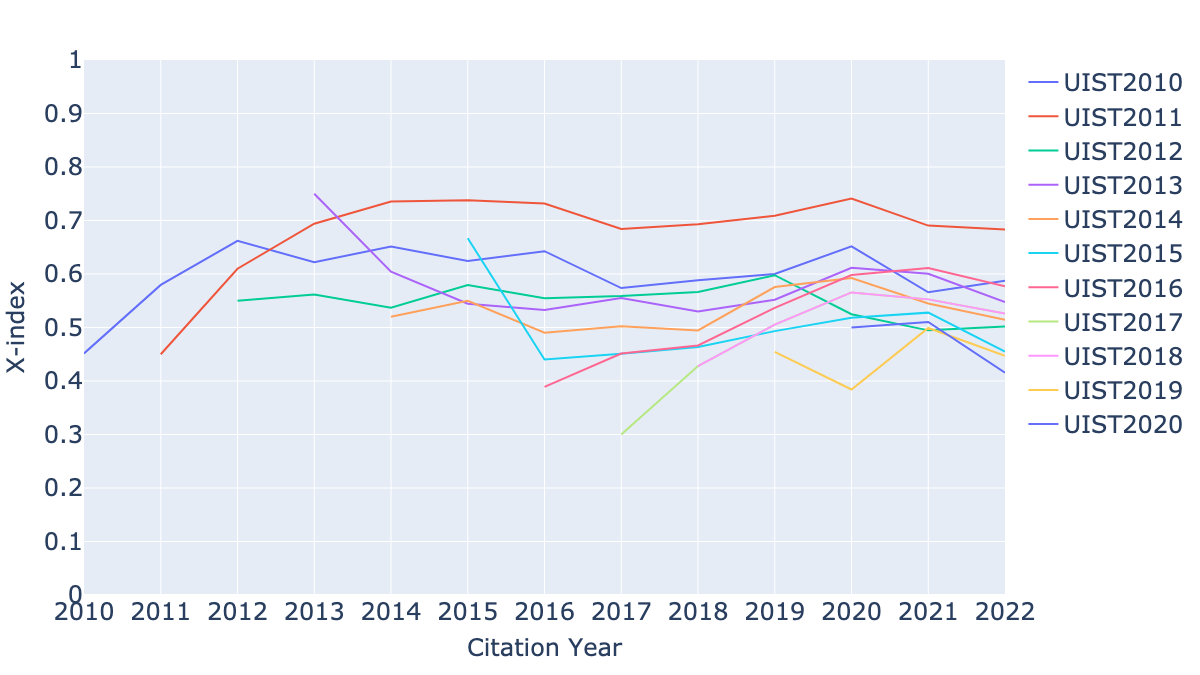
\includegraphics[width=\columnwidth]{figures/fig3_UIST.png}
    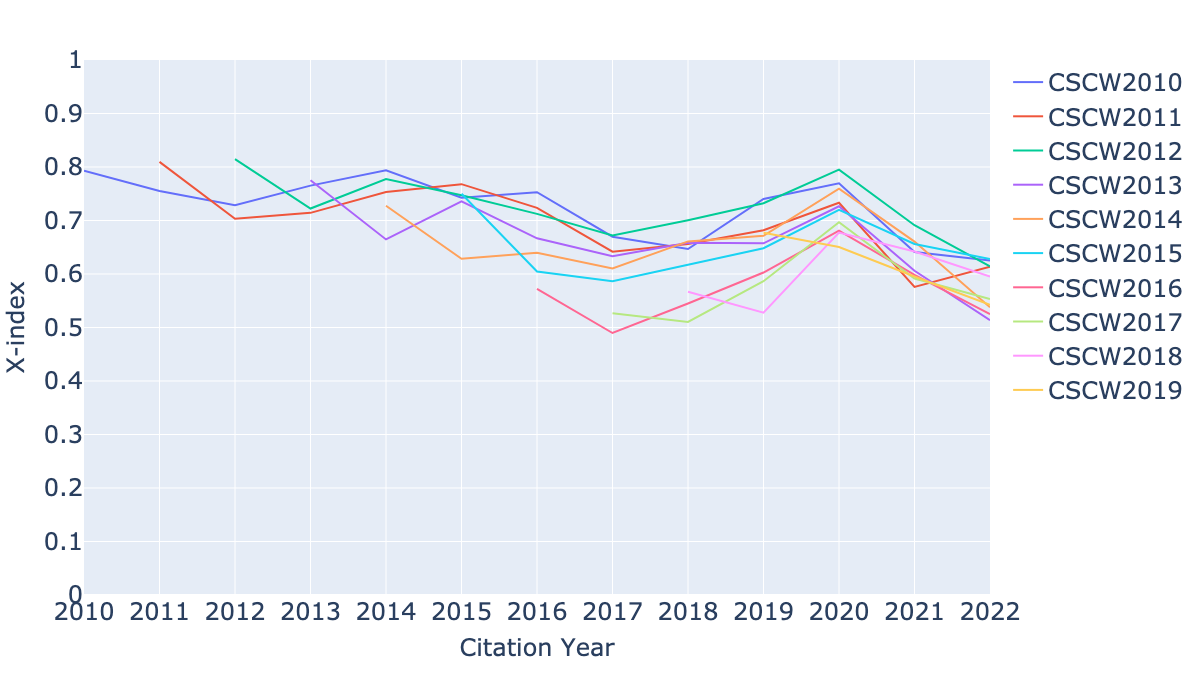
\includegraphics[width=\columnwidth]{figures/fig3_CSCW.png}
    \caption{Amongst all the HCI papers cited in a given year, the earlier papers tend to have a higher \xin than the later ones.}
    \label{fg:fig3}
\end{figure}

\subsection{\xin of HCI Papers, Only Counting Citations in the Five Years After Publication}
% One issue of the above analysis is that HCI papers published later (\eg 2019) likely have fewer citations than the earlier ones (\eg 2010) simply because the earlier-published papers existed for a longer period of time.
To balance the playing field, we now consider citations that occurred only within the first five years after an HCI paper was published.
For example, for CHI 2015 papers, we only consider citations of them that occurred between 2016 and 2020.
This constraint narrows the overall analysis down to only HCI papers published from 2010 to 2017 because, later than that, our data (collected in January 2023) has less than five years of citation information.

As shown in \fgref{fig2}, the result indicates that, even accounting for how long an HCI paper has been around, the overall \xin still seems to decrease over the years.



\subsection{\xin Year-by-Year After the Publications of Each Year's HCI Papers}

To further understand the relationship between \xin and how long a paper has been published, we plot each year's published HCI papers' \xin over the subsequent years, as shown in \fgref{fig3}.
% To delve deeper into the previous two analyses and results that show a decreasing \xin of HCI papers, 
% we now break down citations into individual publishing years for each of the three HCI venues.
% For each HCI venue on a particular year (\eg CSCW 2014), we plot the \xin for each of the subsequent year (including the publication year, \eg 2014-2022 for CSCW 2014), as shown in \fgref{fig3}.

Note that the $x$-axis in \fgref{fig3} has changed: it is now citation year, not publication year. For example, when some papers in 2019 cite a CSCW 2013 paper, the citation year is 2019 whereas 2013 is the publication year.
The results show that, for most years' HCI papers, their \xin tends to flatten or slightly decrease over time, except for a few `local' cases, \eg UIST 2011's \xin kept increasing until 2014.

Amongst HCI papers cited in a given citation year, the earlier papers tend to have a higher \xin than the later ones. 
Consider the year 2020. 
For CHI, the top-3 \xin in 2020 are papers published in 2010, 2011, and 2015 whereas the bottom-3 are 2019, 2018, and 2017;
For UIST, the top-3 \xin in 2020 are papers published in 2011, 2010, and 2013 whereas the bottom-3 are 2019, 2020, and 2012;
For CSCW, the top-3 \xin in 2020 are papers published in 2012, 2010, and 2014 whereas the bottom-3 are 2019, 2018, and 2016.

\fg{fig4}{fig4}{1.0}{In the more recent years, HCI papers seem less likely to be cited by papers outside of our core HCI venue list.}

\subsection{\xin of HCI Papers Cited Over the Years}

The previous analysis suggests that we can aggregate each year's citations of HCI papers so that we can see how the non-HCI papers' interest in citing HCI papers changed over the years.

For each year, we consider that year's citations of HCI papers published in previous five years.
Since our HCI papers start earliest in 2010, our analysis can only begin from 2015 (A 2014 paper might cite a CHI 2009 paper but we do not have CHI 2009's citation information in our dataset).

\fgref{fig4} shows the results, which also exhibit a decreasing pattern over the years.
In other words, in the more recent years, HCI papers seem less likely to be cited by papers outside of our core HCI venue list.

